% sanas_apc.tex -- Sanas engineering paper: single-chip 64-zone ToF as a bus APC.
% IEEE conference format. Draft written 2026-08-10 by Danyshpan from logged,
% completed results only (experiments/log.md, docs/findings.md,
% docs/trade_study.md, paper/results/apc_validation.{md,json}).
%
% FIGURES: built by CADy to the specification in paper/figures.md.
% Result plots (Figs. 1-3) are generated from paper/results/apc_validation.json.
% Hardware figures (Figs. 4-7) are PDF exports of the existing SVGs in
% docs/hardware/figures/. Do not renumber figures without updating figures.md.
%
% CITATION VERIFICATION STATUS: see the TODO comments in the bibliography.
% Numbers marked "reported" in the text are inferred from abstracts or from
% secondary literature and were not confirmed from full text; numbers marked
% "vendor-claimed" are manufacturer statements with no independent measurement.

\documentclass[conference]{IEEEtran}
\usepackage{cite}
% Figure PDFs are in paper/figures/ (built by CADy per paper/figures.md).
\usepackage{graphicx}
\usepackage{array}
\usepackage{booktabs}
\usepackage{url}
\usepackage{amsmath}

\begin{document}

\title{Counting Bus Passengers with a Single-Chip 64-Zone Time-of-Flight Sensor:\\
A Resolution Ablation on In-Cabin Depth Data}

% TODO: confirm author list, affiliations and order with Diyas before submission.
\author{
\IEEEauthorblockN{Diyas Tleukin}
\IEEEauthorblockA{Sanas Project\\
Almaty, Kazakhstan\\
tleukindias@gmail.com}
% TODO: add co-authors / advisor / institutional affiliation if applicable.
}

\maketitle

\begin{abstract}
Commercial automatic passenger counting (APC) units for buses are door-mounted
depth sensors whose vendor-claimed accuracies of 98 to 99 percent have been
measured as low as 53 percent in field service. We ask whether the opposite end
of the cost scale, a single-chip 64-zone time-of-flight ranging sensor of the
ST VL53L7CX class with a component cost in the single-digit US dollar range,
can serve as a bus APC. We implement a geometric counting pipeline consisting
of depth deprojection, background subtraction, centroid tracking, and
virtual-line crossing, and validate it on a public multi-view in-cabin bus
dataset, simulating the target sensor by pooling an 848$\times$480 depth
stream to 8$\times$8 and 4$\times$4 zone grids. On 25 staged boarding and
alighting episodes, the 8$\times$8 simulation detected 24 of 25 (96\%, 95\% CI
80 to 99), assigned all 24 detected directions correctly, produced zero false
positives on negative segments, and tracked the cumulative on-board count with
a mean absolute error of 0.17 against door-event truth. Under identical
untuned parameters it outperformed the full-resolution pipeline (19 of 25),
which loses line-hover episodes to depth-noise cluster fragmentation that
coarse pooling suppresses; the 4$\times$4 grid falls below the working floor.
We additionally report a measured negative result for cabin-wide oblique depth
occupancy (10\% floor coverage, $r=0.184$, non-monotonic beyond two occupants)
that motivates door counting over cabin-wide sensing, a deployment-geometry
finding that forces the counting line into the vestibule at a measured
accuracy cost, and a distributed node design with terminus reset and an
ordinal crowding output for a rider-facing application. With $n=25$ staged
episodes on substitute data, these results indicate feasibility only; no
compliance with counting standards such as VDV 457 can be claimed.
\end{abstract}

\begin{IEEEkeywords}
automatic passenger counting, time-of-flight sensing, depth sensing, public
transport, edge computing, occupancy estimation
\end{IEEEkeywords}

\section{Introduction}
\label{sec:intro}

Automatic passenger counting underpins service planning, revenue allocation,
and, increasingly, real-time crowding information shown to riders before they
board. The commercial state of the art is a door-mounted 3D depth unit; vendors
in this segment claim counting accuracies of 98 to 99 percent
\cite{irma,dilax}, and in Germany acceptance of APC systems is governed by the
VDV~457 recommendation \cite{vdv457}, whose validation methodology bounds
systematic error at $\pm$1\% (as reported in the validation literature
\cite{ellenberger2023}).

Two problems limit the reach of these systems. First, cost: commercial APC
units occupy the high end of the market, with unit prices unpublished by any
major vendor, and instrumenting every door of a large municipal fleet is a
significant procurement. Second, the gap between claim and field: in the only
independent field study we found, a commercial video-based APC unit claimed at
98\% by its vendor measured 53.17\% (boarding) and 55.29\% (alighting) over 20
days of revenue service \cite{pronello2023}. Both problems motivate examining
the extreme low-cost end of the depth-sensing spectrum with measured, not
claimed, numbers.

Depth-based counting at transit doors is well established: LSTM counters on
low-resolution 3D LiDAR over train doorways report approximately 96\% correct
door-phase counts \cite{seidel2021} (reported), a CNN-LSTM on time-of-flight
(ToF) depth above train doors reports 99.79\%/99.97\% boarding/alighting
accuracy \cite{seo2026} (reported), dense stereo over a bus door reached
99\%/97\% on two datasets as early as 2010 \cite{yahiaoui2010}, and a public
RGB-D bus-entrance dataset exists \cite{sun2019}. Low-resolution ToF counting
is likewise established outside transit, in office occupancy \cite{lu2021} and
doorway counting \cite{jeong2025}, and embedded ToF counting has been proposed
for public transport \cite{stec2019}. What the literature does not contain, to
our knowledge, is an ablation of depth resolution down to the single-chip
multizone grid (8$\times$8 zones, 90$^\circ$ diagonal field of view, 15\,Hz
maximum in 8$\times$8 mode \cite{st_vl53l7cx}) on transit-cabin data, nor a
treatment of what happens to APC geometry when the assumed top-down aperture
view is not available.

This paper asks a narrow question: can a VL53L7CX-class 64-zone ToF sensor
serve as a bus APC? We answer it by simulation on the only public multi-view
in-cabin bus depth dataset we could obtain \cite{gorelik2026}, and we report
the answer with its uncertainty intact. The contributions are:
\begin{enumerate}
  \item a resolution-ablation study (full 848$\times$480 depth versus
        simulated 8$\times$8 and 4$\times$4 zone grids) of virtual-line door
        counting on transit-cabin depth data, in which the 8$\times$8
        simulation outperformed full resolution under identical untuned
        parameters, with the mechanism diagnosed;
  \item a measured deployment-geometry finding: an oblique in-cabin rig cannot
        reproduce top-down aperture geometry, forcing the counting line into
        the vestibule, and the cost of that placement is quantified;
  \item a measured negative result for cabin-wide oblique depth occupancy
        (10\% floor coverage, $r=0.184$, non-monotonic beyond two occupants)
        as evidence for door counting over cabin-wide depth sensing;
  \item a system design for distributed low-cost ToF nodes with a CAN trunk,
        gateway counting, terminus reset, and a five-level ordinal crowding
        output, with a designed but deliberately untrained RGB drift
        corrector.
\end{enumerate}
We do not claim the first low-resolution ToF people counter, nor the first
depth APC at transit doors; both exist \cite{lu2021,jeong2025,stec2019,%
seidel2021,seo2026,yahiaoui2010}. We claim the ablation, the geometry finding,
the negative result, and the design.

\section{Related Work}
\label{sec:related}

\subsection{Depth-Based APC at Transit Doors}

Door counting at the chokepoint, rather than sensing the whole cabin volume,
is the shape the commercial industry converged on \cite{irma,dilax}.
Yahiaoui et al. demonstrated dense-stereo bus-door counting with 99\% and 97\%
accuracy on two datasets \cite{yahiaoui2010}. Seidel et al. published NAPC, an
LSTM on low-resolution 3D LiDAR depth over train doorways with roughly 13{,}000
annotated recordings and approximately 96\% correct door-phase counts
(reported) \cite{seidel2021}. Seo et al. report a CNN-LSTM on ToF depth above
train doors at 99.79\%/99.97\% boarding/alighting and state compliance with
the $\pm$1\% VDV~457 requirement (reported) \cite{seo2026}; notably, that work
also spatially downsamples 2D video for privacy, which partially overlaps our
resolution-ablation idea but operates on grayscale video rather than depth
grids. Sun et al. released PCDS, a public RGB-D dataset recorded at bus
entrance doors \cite{sun2019}; its CC~BY-NC-SA licence restricts it to
non-commercial use, which is one reason our system design retains raw frames
as future licence-clean training data (Sec.~\ref{sec:system}). Pronello and
Garz\'on Ruiz provide the field-reality anchor for this literature: a
vendor-claimed 98\% system measured at 53--55\% in service, against 72--75\%
for the authors' own low-cost build \cite{pronello2023}. Regionally, RGB video
counting with detector-tracker pipelines has also been applied to passenger
counting in Kazakhstan \cite{nurseitov2026}.

\subsection{Low-Resolution and Low-Cost Grid Sensors}

Sparse and low-resolution ToF sensing for people counting predates this work.
Lu et al. used a sparse array of low-resolution ToF sensors for zone-level
office occupancy with a reported error rate near 0.4\% \cite{lu2021}
(reported). Jeong et al. mounted a ToF camera above a doorway and report over
90\% accuracy for single-entry/exit scenarios with a privacy framing similar
to ours \cite{jeong2025} (reported). Stec et al. proposed embedded ToF people
counting explicitly for public transport \cite{stec2019}. The closest
cheap-grid-on-microcontroller system we found uses a low-resolution thermal
array on an ESP32 \cite{papanashi2026} (reported). None of these ablate depth
resolution down to a single-chip 64-zone grid on transit-cabin data, which is
the specific gap this paper addresses.

\subsection{Alternative Modalities}

An internal trade study compared depth against mmWave radar, CO$_2$, Wi-Fi/BLE
probe counting, thermal arrays, and IR beam-break pairs. mmWave people
counting reports strong results in familiar environments but degrades in
unseen ones and struggles with stationary subjects \cite{toha2025} (reported);
CO$_2$-based counting responds minutes after occupancy changes, incompatible
with 20--60\,s stop-to-stop dynamics \cite{ariefang2017} (reported). Probe
counting is defeated by MAC randomization and needs observation windows far
longer than a stop, and thermal arrays lose contrast when summer cabin
temperatures approach body temperature; both were rejected in the trade study
on those grounds. Depth at the door remained the strongest published modality
for this task.

\section{Substitute Dataset and Its Limits}
\label{sec:dataset}

No in-cabin camera data of our own exists yet (municipal approval pending), so
the study uses the multi-view in-cabin dataset of Gorelik et al.
\cite{gorelik2026} (73.5\,GB, CC~BY~4.0, Zenodo
DOI \texttt{10.5281/zenodo.20559664}): four RGB-D camera rigs and a LiDAR in a
German urban bus. The depth streams are 848$\times$480 (one camera
640$\times$480) with per-camera intrinsics and full extrinsic chains published
in the archive. The sensor model is not named in the archive; the
848$\times$480 depth mode is characteristic of the Intel RealSense D400
series, and we treat the D435i identification as an inference, not a fact.

The dataset's limits shape everything downstream and are stated up front. It
is a single 32-minute staged daytime session (2026-05-21) with actors, in a
stationary vehicle, split into 11 sub-sequences. The per-frame occupant
distribution over 9{,}975 frames is $\{1{:}\,4989,\ 2{:}\,4418,\ 3{:}\,546,\
4{:}\,22\}$ with 26 unique person identities and 898 empty-cabin frames; the
cabin never holds more than four people. Annotations are pseudo-labels
produced by an automated pipeline with manual filtering; only the per-person
state and action labels are hand-made. There is no night or artificial-light
data, no vehicle motion, and no route, terminus, or GPS metadata.

Ground truth for counting comes from the hand-made state labels: the states
\emph{enter vehicle} (377 frames) and \emph{exit vehicle} (436 frames),
grouped into contiguous episodes per person with a 2\,s gap tolerance, yield
\textbf{25 episodes (12 boardings, 13 alightings)} across the session, with a
median episode length of 31 frames (about 3\,s). These 25 events, involving
roughly nine distinct persons, one of whom contributes eight episodes, are the
entire validation set. Every detection is worth 4 percentage points of
accuracy. All confidence intervals in this paper exist because of this.

\section{Cabin-Wide Depth Occupancy: A Negative Result}
\label{sec:negative}

The project's original plan was cabin-wide occupancy estimation from in-cabin
depth. We report its measured failure because it motivates the door-counting
architecture and because negative results at this level of specificity are
rare in the APC literature.

The method is purely geometric: deproject each depth frame with the camera's
own depth intrinsics (using colour intrinsics silently fails, as the focal
lengths differ by more than 2$\times$), transform into the vehicle frame,
accumulate a bird's-eye-view occupancy grid (0.1\,m cells, height band 0.6 to
2.0\,m), subtract a background built from empty-cabin frames, and score each
frame by its occupied-cell fraction. The score was correlated against the
pseudo-label occupant count on $n=1{,}204$ frames from the front-left depth
camera.

\begin{table}[t]
\caption{Cabin-wide BEV occupancy score by ground-truth occupant count
(front-left depth camera, $n=1{,}204$ frames). The score is the fraction of
grid cells occupied. It is not monotonic in the count.}
\label{tab:bev}
\centering
\begin{tabular}{ccccc}
\toprule
Count & $n$ & Mean & Median & Std \\
\midrule
0 & 118 & 0.0014 & 0.0013 & 0.0003 \\
1 & 615 & 0.0017 & 0.0015 & 0.0007 \\
2 & 412 & 0.0019 & 0.0015 & 0.0010 \\
3 & 59  & 0.0017 & 0.0014 & 0.0009 \\
\bottomrule
\end{tabular}
\end{table}

Three independent measurements condemn the approach. First, coverage: against
the region occupants actually use (4{,}110 cells derived from every 3D box in
the recording, dilated 0.3\,m), the camera's depth returns inside its reliable
0.3 to 3.0\,m window cover \textbf{10.0\%} of the region; only 42.2\% of all
depth pixels fall inside that window at all, and a preliminary four-camera
union reaches only 28.8\% at spec range (30-frame sample; indicative, not
sanctioned). Second, correlation: Pearson $r=0.184$ (95\% CI $[0.133,
0.231]$), Spearman $\rho=0.139$ ($[0.081, 0.199]$); the association excludes
zero and explains about 3\% of the variance. Third, monotonicity: as
Table~\ref{tab:bev} shows, the mean score rises from zero to two occupants and
falls at three. This is the saturation expected of a surface sensor, which
images the shell of a group rather than its volume, and it appears at three
people rather than thirty. A signal that saturates at exactly the occupancy
levels a crowding product must distinguish is not a usable primary signal.
Counting at the door chokepoint, where the industry converged
\cite{irma,dilax,yahiaoui2010,seidel2021}, is what the evidence supports.

\section{Door Counting Under Oblique-Geometry Constraints}
\label{sec:method}

\subsection{Deployment Geometry: Why the Line Moves Inside}
\label{sec:geometry}

A real APC looks straight down over the door aperture; the top-down view is
what makes line crossing robust to occlusion. Measured from the archive's
extrinsics, none of the dataset's four depth cameras provides such a view:
mount heights are 1.95 to 2.04\,m and optical axes are 67$^\circ$ to
74$^\circ$ off vertical, i.e.\ the rig looks across the aisle, not down
(Finding~A). Of the four cameras, exactly one (\emph{center\_left}) reaches
the door-zone footprint inside the 0.3 to 3.0\,m depth window, with 1{,}746
in-range points per frame at 2.05 to 2.77\,m; the other three see the
zone only beyond 3.6\,m (Finding~B). Finally, the labelled crossing positions
themselves are unusable: at the first frame of an entry (or last frame of an
exit) the person is still on the kerb, 3.24 to 5.96\,m from the camera and
outside the reliable window. However, all 25 of 25 boarding and alighting
trajectories pass through the camera's usable zone inside the cabin, with
closest approach 1.22 to 2.24\,m (Finding~C).

The consequence is a deployment finding, not a preference: with this geometry
the virtual counting line cannot lie across the door aperture and must be
placed \emph{inside the cabin}, in the vestibule. This deviates from the APC
pattern the literature assumes, and Sec.~\ref{sec:results} quantifies its
cost. The finding generalizes beyond this dataset: any oblique retrofit
camera, which is the cheapest thing to install in an existing vehicle, faces
the same constraint.

\subsection{Counting Pipeline}

The counter is geometric, with no learned component. Per frame: (1)~deproject
the depth image with the camera's own intrinsics (848$\times$480,
$f_x \approx 426.6$) and transform points into the vehicle frame using the
archive's extrinsic chain; (2)~restrict to a door zone ($x \in [-0.6, 1.6]$,
$y \in [-0.2, 1.3]$, $z \in [0.2, 2.0]$\,m) and to ranges 0.3 to 3.0\,m;
(3)~subtract a static background (per-pixel median over 48 empty-cabin frames,
margin 0.15\,m); (4)~cluster foreground points on a 0.15\,m grid with a
60-point minimum and take cluster centroids; (5)~associate centroids to tracks
by nearest neighbour (gate 0.8\,m, maximum track gap 0.7\,s); (6)~count a
boarding or alighting when a track crosses the virtual line at $x=0.20$\,m
with a hysteresis band of $\pm$0.15\,m. The cumulative on-board count is
$N_t = N_{t-1} + \text{boardings} - \text{alightings}$. Every parameter is an
untuned default chosen from geometry inspection before any result was
computed, and none was adjusted afterwards; with 25 validation events, tuning
against the validation set would corrupt it (Sec.~\ref{sec:limitations}).

\subsection{Simulating the 64-Zone Sensor}

The VL53L7CX provides an 8$\times$8 grid of range values over a
60$^\circ\times$60$^\circ$ square field of view at up to 15\,Hz in 8$\times$8
mode (60\,Hz in 4$\times$4) \cite{st_vl53l7cx}. We simulate it by cropping the
depth frame to a central 60$^\circ\times$60$^\circ$ field (vertically limited
by the source camera's $\approx$58$^\circ$ field) and pooling each block to
its 20th-percentile valid range, yielding an 8$\times$8 (and, for the
ablation, 4$\times$4) zone-range grid per frame. The zone grid then passes
through the identical downstream logic (deprojection of zone rays, background
subtraction with 0.2\,m margin, clustering at 0.4\,m, the same tracker and
line). Processing ran at every second frame ($\approx$7.7\,Hz of the nominal
15.4\,Hz stream), inside the frame-rate class of the real sensor; a 15\,Hz
spot check on three episodes produced identical event streams.

The simulation inherits the source camera's stereo noise model, not the
VL53L7CX's ToF noise; the two differ in kind, notably in sunlight. This is a
stated fidelity limit (Sec.~\ref{sec:limitations}), not a footnote.

\subsection{Validation Protocol}

From the session we processed 2{,}167 frames in 21 episode chunks (buffers
$-2/{+}5$\,s around boardings and $-5/{+}2$\,s around alightings, asymmetric
per the measured crossing-time distribution), six negative chunks totalling
63\,s with no door event, and the 48 background frames. An episode counts as
detected if at least one crossing event falls in a $\pm$6\,s match window;
direction is scored on the first event in the window. All counts are anchored
at zero at the first processed frame; because actors already aboard at the
anchor alight later, door-event truth spans $-4$ to $+1$ and ends the session
at $-1$. Proportions carry Wilson 95\% intervals and the false-positive rate
a Garwood (Poisson) interval. $N_t$ MAE is computed over the 2{,}167
processed frames only (outside processed chunks the estimate is frozen
across intervals the counter never observed), with a block-bootstrap 95\%
interval over chunks.

\section{Results}
\label{sec:results}

\begin{table}[t]
\caption{Virtual-line counting across sensor resolutions, $n=25$ episodes
(12 board, 13 alight). Wilson 95\% CIs for proportions; Garwood interval for
the FP rate; block bootstrap over chunks for MAE, computed over the 2{,}167
processed frames. Final $N_t$ errors are evaluated at the last processed
frame. Every episode is worth 4 percentage points.}
\label{tab:headline}
\centering
\setlength{\tabcolsep}{4pt}
\begin{tabular}{lccc}
\toprule
 & Full 848$\times$480 & 8$\times$8 sim & 4$\times$4 sim \\
\midrule
Episodes detected & 19/25 & \textbf{24/25} & 21/25 \\
\quad (rate, 95\% CI) & 76\% [57, 89] & \textbf{96\% [80, 99]} & 84\% [65, 94] \\
Direction correct & 19/19 & 24/24 & 18/21 \\
Duplicate events & 1 & 0 & 5 \\
FP on 63\,s negatives & 0 & 0 & 0 \\
\quad (upper 95\%, min$^{-1}$) & 3.49 & 3.49 & 3.49 \\
$N_t$ MAE vs.\ door truth & 1.45 & \textbf{0.17} & 1.92 \\
\quad (95\% CI) & [1.08, 1.91] & [0.11, 0.26] & [1.47, 2.37] \\
Final $N_t$ error (door) & $-3$ & $+1$ & $+3$ \\
$N_t$ MAE vs.\ line truth & 2.83 & 1.53 & 0.93 \\
Detected excl.\ person~1 & 11/17 & 16/17 & 14/17 \\
\bottomrule
\end{tabular}
\end{table}

Table~\ref{tab:headline} is the headline; Fig.~\ref{fig:nt} shows the
cumulative count against both truth references over the session, and
Fig.~\ref{fig:ablation} summarizes the ablation with its intervals.

\begin{figure*}[t]
\centering
% Built by CADy from apc_validation.json (nt.*.series_1hz + per_episode).
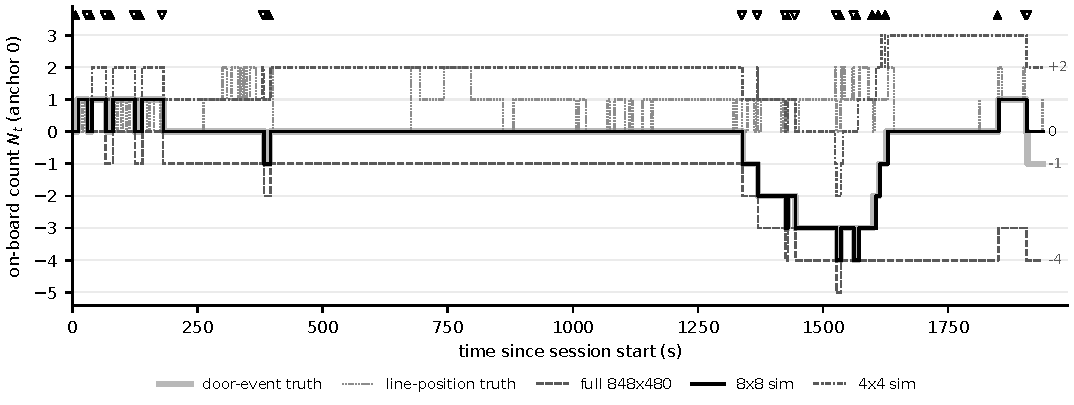
\includegraphics[width=\textwidth]{figures/fig1_nt_series.pdf}
\caption{Cumulative on-board count $N_t$ at 1\,Hz for the full-resolution
pipeline and the 8$\times$8 and 4$\times$4 zone simulations, against two
references: door-event truth (bold staircase; the 25 labelled episodes
applied at episode midpoints) and line-position truth (dotted; persons on the
cabin side of the line plane, which moves whenever anyone crosses it, door
event or not). All counts are anchored at zero at the first processed frame,
so door-event truth dips to $-4$: actors already aboard, whose boarding was
never observed, alight later. Markers on the upper edge give labelled
boarding (up) and alighting (down) episodes; estimates freeze outside
processed chunks. Session-end door-event truth is $-1$ against estimate
endpoints of $0$ (8$\times$8), $-4$ (full), and $+2$ (4$\times$4), giving the
final errors $+1$, $-3$, $+3$ of Table~\ref{tab:headline}. MAE values are
computed over the 2{,}167 processed frames, not this 1\,Hz display grid.}
\label{fig:nt}
\end{figure*}

\begin{figure}[t]
\centering
% Built by CADy from apc_validation.json (variants.* + nt.*).
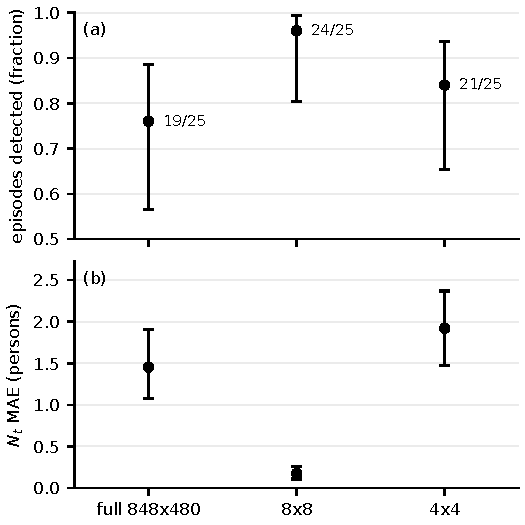
\includegraphics[width=\columnwidth]{figures/fig2_resolution_ablation.pdf}
\caption{Resolution ablation on $n=25$ episodes. (a)~Episode detection rate
with Wilson 95\% intervals. (b)~Cumulative-count MAE against door-event truth
with block-bootstrap 95\% intervals. The 8$\times$8 simulation outperforms
full resolution under identical untuned parameters; every episode is worth 4
percentage points, so the intervals are the honest summary.}
\label{fig:ablation}
\end{figure}

\subsection{The 8$\times$8 Simulation Beats Full Resolution, and Why}

Under identical untuned defaults the 8$\times$8 simulation detected 24/25
episodes against full resolution's 19/25, with a cumulative-count MAE of 0.17
against 1.45. The mechanism is diagnosed, not guessed. Full resolution misses
exactly the six episodes in which a person hovers on the counting line: in one
traced episode the centroid sits within 0.03\,m of the line plane for more
than 3\,s. At the crossing instant, depth noise fragments the person's point
cloud into multiple clusters; the greedy tracker births a new track on the
cabin side, and the crossing is attributed to no track. Pooling to 8$\times$8
zones spatially regularizes the person to a single centroid, and the same
crossing is counted cleanly. This is a genuine property of the untuned
full-resolution clustering (0.15\,m cells, 60-point minimum), not a code
defect; coarser full-resolution clustering would likely recover the episodes,
but any tuning against the only 25 events would corrupt the validation set, so
the failure is left measured and unfixed. The honest framing is therefore
narrow: \emph{on this data, spatial pooling to the sensor-grid resolution
acted as regularization for door counting; the low-cost 64-zone simulation did
not degrade counting, it improved it under these defaults.} We do not claim
the ordering would survive tuning of the full-resolution path.

\subsection{4$\times$4 Is Below the Working Floor}

Detection at 4$\times$4 holds at 21/25, but three direction errors and five
duplicate events appear: at two zones' width, a person straddling the line
chatters across it. In this geometry 8$\times$8 is the working minimum;
4$\times$4 is not. This bounds how far the cost floor can be pushed.

\subsection{The Cost of the Vestibule Line}

Line-crossing counts and door-event counts are different quantities on this
data. The line-position truth (persons on the cabin side of the plane, from
the 3D boxes) moves between episodes without any door event: an actor using a
wheelchair, already aboard, crosses the vestibule plane during internal
circulation, visible in Fig.~\ref{fig:nt} where line-position truth moves
while door-event truth is flat. A deployed vestibule-line counter counts such
crossings; a
door-aperture APC would not. On this recording the gap dominates the
line-truth error (8$\times$8: MAE 1.53 against line truth versus 0.17 against
door truth). This is the measured price of the Finding~C placement that pure
aperture geometry does not pay. A deployment must either shape the counting
zone so internal circulation cannot clip it, or accept that $N_t$ tracks
``cabin side of the line'' rather than ``aboard.''

\subsection{Counting-Band Width}

\begin{figure}[t]
\centering
% Built by CADy from apc_validation.json (band_ablation).
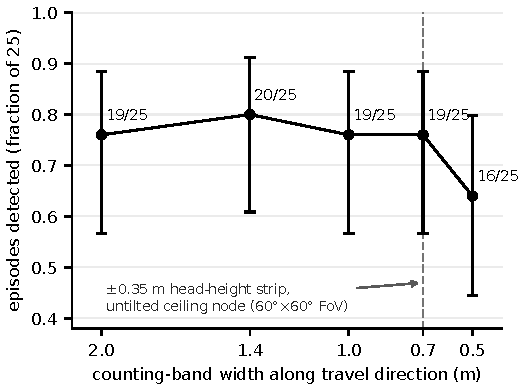
\includegraphics[width=\columnwidth]{figures/fig3_band_sweep.pdf}
\caption{Detection against counting-band width (full-resolution path, zone
truncated to $|x - x_{\mathrm{line}}| \le w$; band width $2w$). Detection is
flat down to a 0.7\,m band and collapses at 0.5\,m, where the $\pm$0.15\,m
hysteresis leaves only 0.1\,m of visible approach per side. The reference
line at 0.7\,m marks the $\pm$0.35\,m head-height strip of an untilted
ceiling-mounted node (60$^\circ\times$60$^\circ$ field of view), which sits
exactly at the measured working minimum with no margin.}
\label{fig:band}
\end{figure}

For mounting design we swept the zone width along the direction of travel
(Fig.~\ref{fig:band}): detection is flat at 19--20/25 for band widths from
2.0\,m down to 0.7\,m and collapses to 16/25 at 0.5\,m, where the $\pm$0.15\,m
hysteresis leaves tracks only 0.1\,m of visible approach on each side of the
line, too little to establish a side before crossing. The effective counting
band must be at least about 0.7\,m wide in the direction of travel. This
number feeds directly into the node mounting geometry
(Sec.~\ref{sec:system}): a face-down node with the sensor's
60$^\circ\times$60$^\circ$ field of view on a 2.3\,m ceiling covers a
$\pm$0.35\,m strip at head height, exactly the measured 0.7\,m minimum with
no margin, so the node must either be tilted, mounted inboard, or detect at
torso/floor level. The caveat carries over: the sweep was measured on an oblique view
narrowed in the vehicle frame, not on a real ceiling footprint.

\subsection{Shared Failure Case}

Every variant merged the one back-to-back double exit (two persons crossing
0.1\,s apart) into a single event; it is the 8$\times$8 simulation's only
miss. Simultaneous crossings remain the known hard case of line-based
counting, consistent with the beam-break and APC literature, and the dataset
contains at most two people simultaneously at the line, so crowded-door
behaviour is unobserved.

\section{System Design}
\label{sec:system}

The measured results above fix the architecture of the deployable system,
shown in Fig.~\ref{fig:arch}. Nothing in this section has been built or
validated on hardware; assumptions are marked.

\begin{figure}[t]
\centering
% CADy: export docs/hardware/figures/system_architecture.svg to PDF.
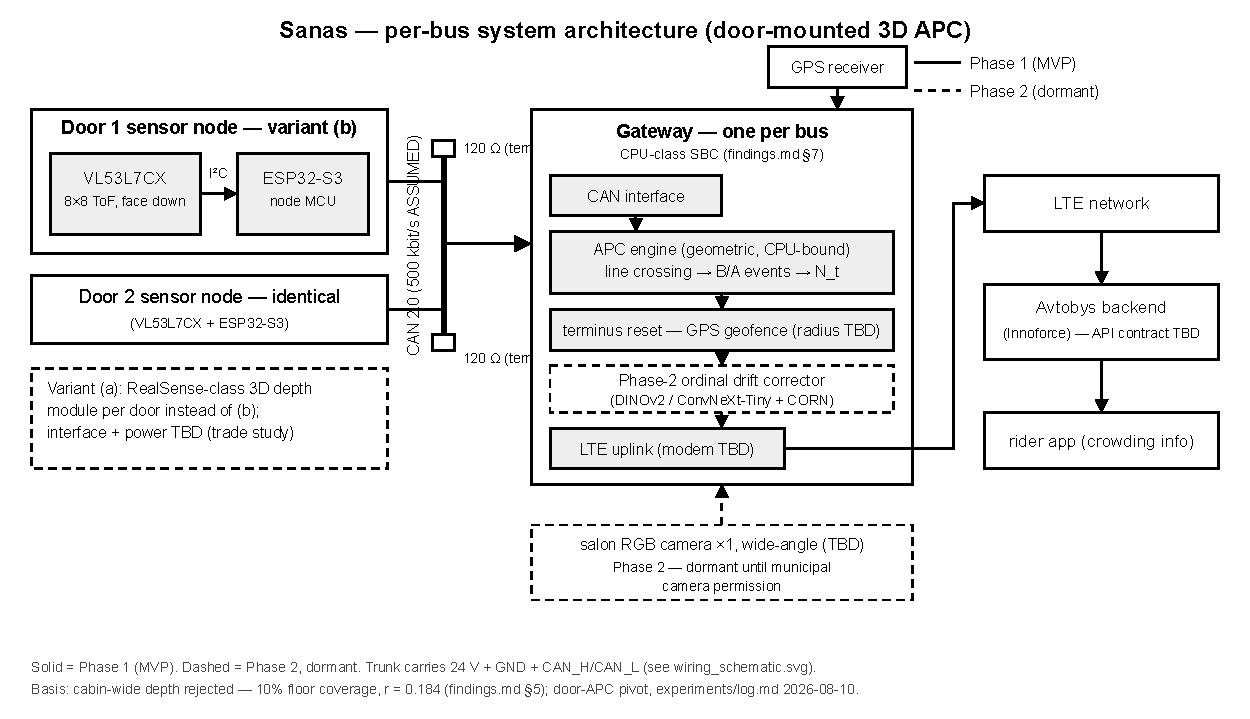
\includegraphics[width=\columnwidth]{figures/fig4_system_architecture.pdf}
\caption{Per-bus system architecture. Two door nodes (VL53L7CX on I$^2$C to an
ESP32-S3) stream raw 8$\times$8 frames over a terminated CAN~2.0 trunk to a
gateway running the geometric counting engine, GPS terminus reset, and LTE
uplink to the transit backend. The Phase-2 RGB drift corrector (dashed) is
designed but not trained.}
\label{fig:arch}
\end{figure}

\begin{figure*}[t]
\centering
% CADy: export docs/hardware/figures/sensor_placement.svg to PDF.
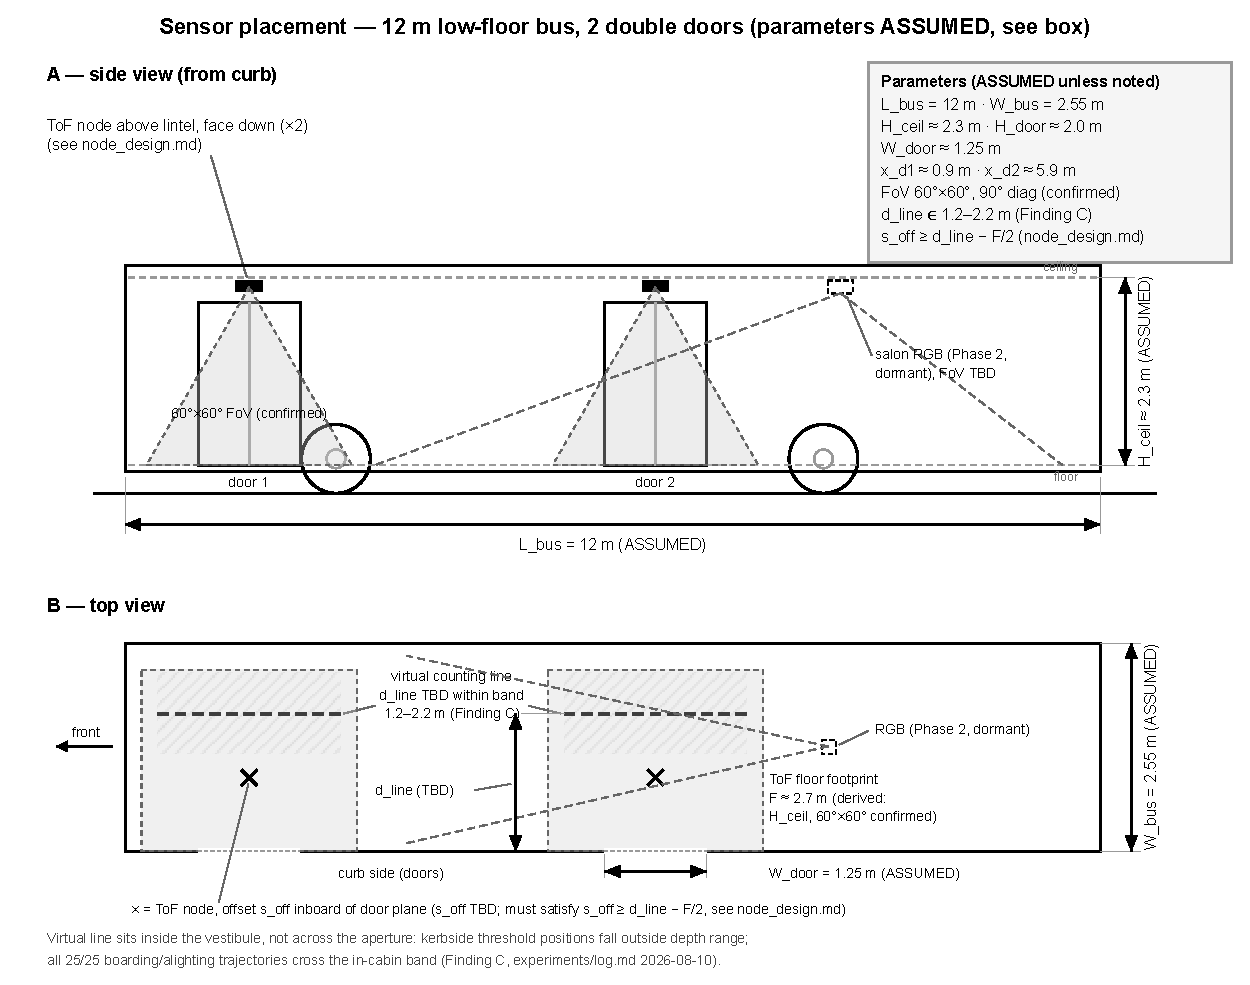
\includegraphics[width=\textwidth]{figures/fig5_sensor_placement.pdf}
\caption{Proposed sensor placement, side (A) and top (B) views of an assumed
12\,m two-door low-floor bus. Each door carries a face-down ToF node above the
lintel; the virtual counting line lies inside the vestibule within the 1.2 to
2.2\,m band measured in Sec.~\ref{sec:geometry}, and the counting-band result
of Fig.~\ref{fig:band} constrains the mount offset or tilt. All dimensions are
parametric assumptions pending a real vehicle survey.}
\label{fig:placement}
\end{figure*}

\subsection{Distributed ToF Nodes over CAN}

Each door carries a face-down node: a VL53L7CX on I$^2$C to an ESP32-S3
microcontroller, streaming raw 8$\times$8 frames to a central gateway over a
CAN~2.0 trunk that also carries 24\,V power in a single four-conductor harness
(Fig.~\ref{fig:wiring}). The node does no counting. Rationale: (1)~the
crossing algorithm stays centrally updatable, and no node-firmware copy can
drift from the gateway implementation; (2)~raw frames retained at the gateway
are the licence-clean training corpus this project otherwise lacks, since the
closest public bus-door dataset is non-commercial-only \cite{sun2019};
(3)~bandwidth is trivial, 64 zones $\times$ 2\,B $=$ 128\,B per frame, about
15.4\,kbit/s per node at the vendor-rated 15\,Hz and roughly 12.5\% of an
assumed 500\,kbit/s bus for two nodes after framing overhead
(Fig.~\ref{fig:dataflow}). CAN was chosen over RS485 for its automotive
pedigree and existing link layer; the bitrate, the ESP32-S3's on-chip CAN
controller, and the transceiver part remain to be verified against datasheets.

\begin{figure*}[t]
\centering
% CADy: export docs/hardware/figures/wiring_schematic.svg to PDF.
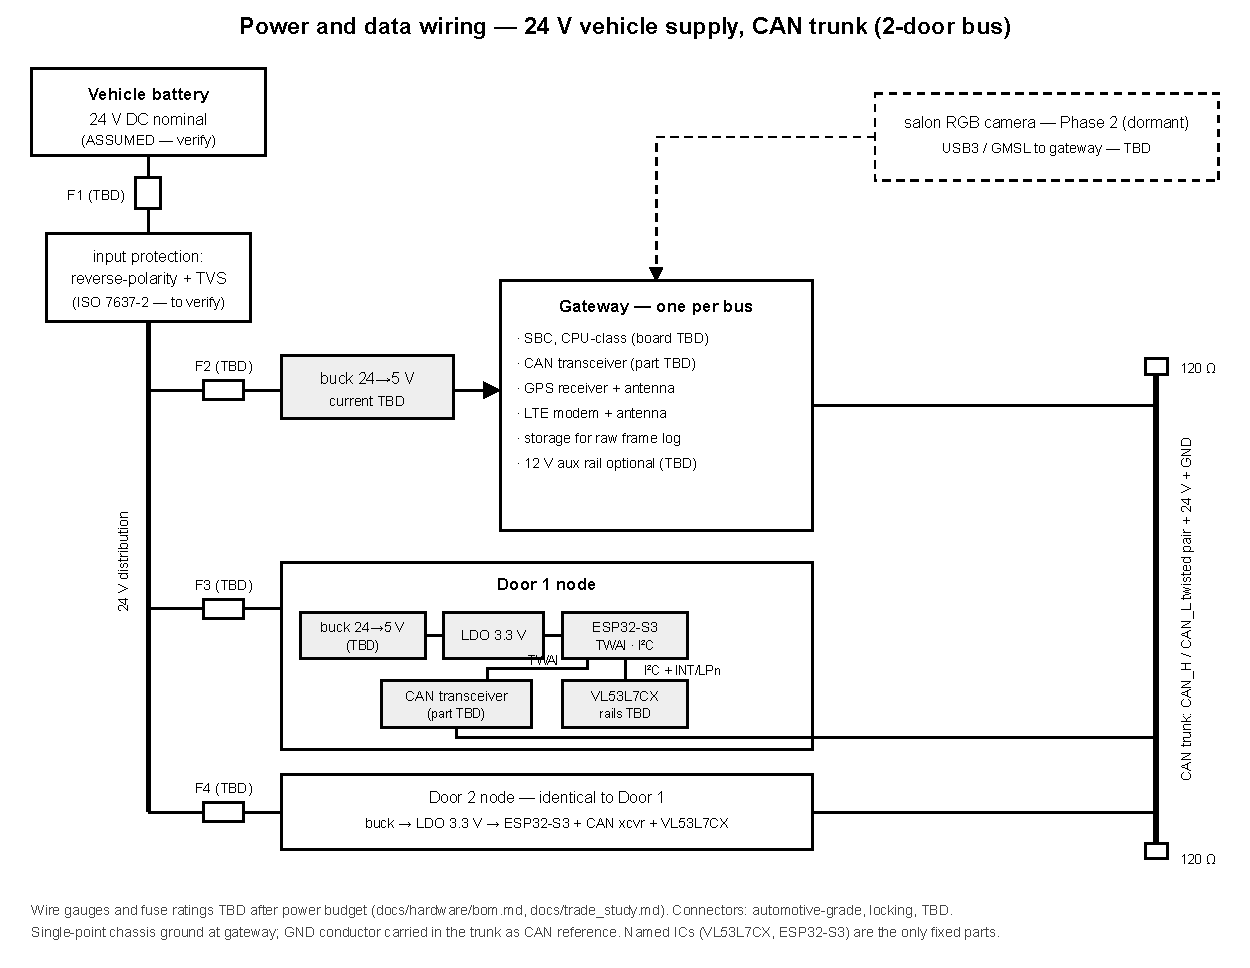
\includegraphics[width=\textwidth]{figures/fig6_wiring_schematic.pdf}
\caption{Power and data wiring for a two-door installation. A fused 24\,V
trunk feeds local buck converters at the gateway and at each node; the CAN
pair is carried in the same four-conductor harness and terminated at both
physical ends. Only the two named ICs are fixed; every rating, gauge, and part
number is an open item (Sec.~\ref{sec:limitations}).}
\label{fig:wiring}
\end{figure*}

\begin{figure*}[t]
\centering
% CADy: export docs/hardware/figures/dataflow.svg to PDF.
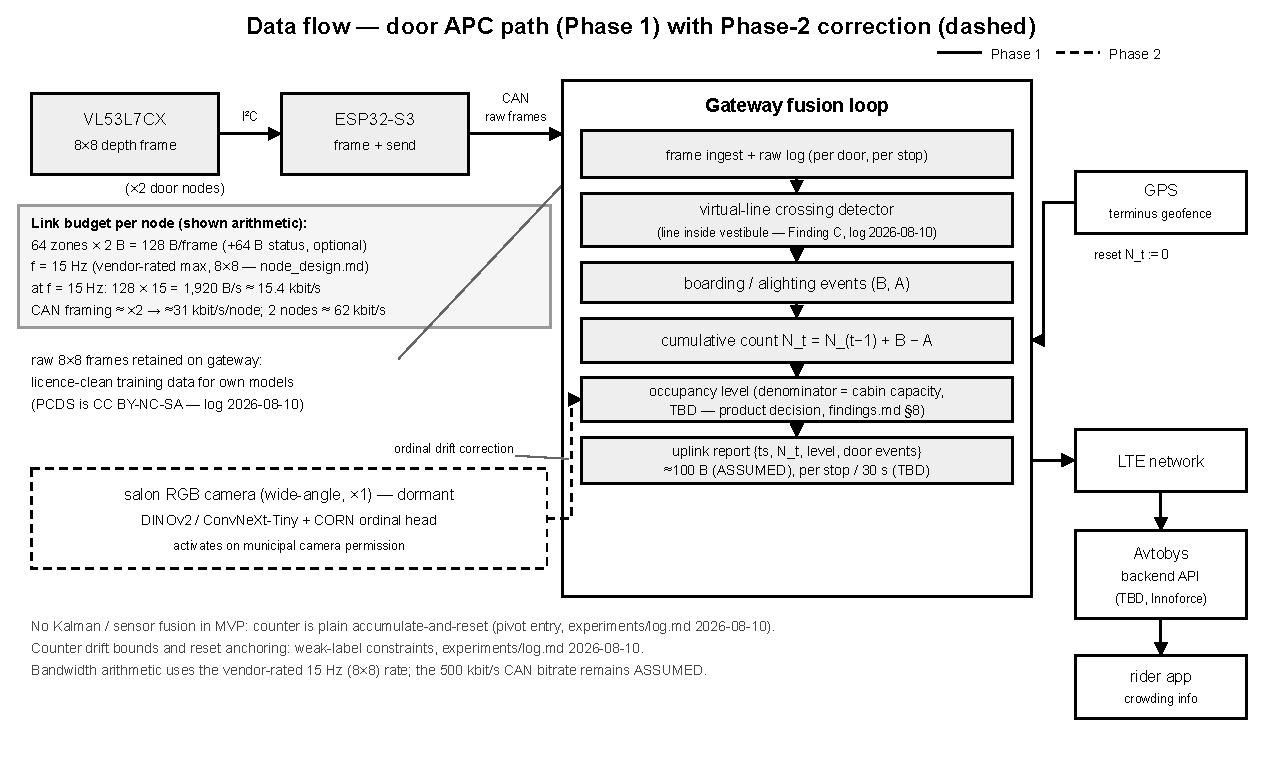
\includegraphics[width=\textwidth]{figures/fig7_dataflow.pdf}
\caption{Data flow with derivable rates. Each node produces
64 $\times$ 2\,B $=$ 128\,B per frame; at the vendor-rated 15\,Hz this is
approximately 15.4\,kbit/s per node before CAN framing, about 12.5\% of a
500\,kbit/s bus for two nodes. Raw frames are retained at the gateway as
licence-clean training data. The Phase-2 ordinal corrector enters dashed.}
\label{fig:dataflow}
\end{figure*}

The privacy argument is structural rather than procedural: 64 range values
per frame cannot image a face, so the primary sensing path collects no
personal data by construction, in the same spirit as the privacy-friendly
train-door work \cite{seidel2021,jeong2025}.

\subsection{Cumulative Count, Terminus Reset, Ordinal Output}

The gateway maintains $N_t = N_{t-1} + b_t - a_t$ with no Kalman filtering or
sensor fusion in the MVP. A cumulative counter drifts without an absolute
anchor; the design's only absolute anchor is a GPS-geofenced terminus reset to
zero. For the rider-facing application (Avtobys), $N_t$ is mapped to a
five-level ordinal crowding scale; the mapping's denominator, cabin capacity,
is a product decision that no public dataset supplies and is deliberately left
open.

\subsection{Phase 2: RGB Ordinal Drift Corrector (Designed, Not Trained)}

What a door counter cannot do is recover from missed events between terminus
resets. For this the design reserves a single salon RGB camera feeding a
frozen self-supervised backbone (DINOv2 ViT-S/14 \cite{oquab2023}, with
ConvNeXt-Tiny \cite{liu2022} as the edge-deployable comparison) and a CORN
ordinal regression head \cite{shi2023} producing periodic absolute crowding
estimates that re-anchor the cumulative count. \textbf{This component is
designed and its loss implementation is unit-checked, but it has not been
trained}: the substitute dataset never exceeds four occupants, so ordinal
levels 3 to 5 have zero training examples, and real cabin data awaits
municipal camera approval. We state this to keep the design honest; no
Phase-2 performance number exists.

\section{Limitations}
\label{sec:limitations}

This section is deliberately long. Each item below bounds what the results can
support.

\textbf{Twenty-five events.} The entire validation set is 25 staged episodes;
one person contributes eight of them. Excluding that person, the 8$\times$8
simulation detects 16/17. A single miscount moves the detection rate by 4
percentage points, which is why every proportion is reported with a Wilson
interval and why we treat the intervals, not the point estimates, as the
result.

\textbf{No VDV 457 claim is possible.} The VDV~457 acceptance methodology
bounds systematic error at $\pm$1\% and, per its validation literature, needs
stratified samples of thousands of door events \cite{vdv457,ellenberger2023}.
Twenty-five events cannot demonstrate or refute compliance in principle. Any
compliance statement requires a revenue-service pilot with manual reference
counts, and this paper makes none.

\textbf{Staged substitute data.} One bus, one door, one 32-minute daylight
session, stationary vehicle, actors following a script. No vibration, no
motion blur, no night, no weather, no doors opening onto sunlight, no real
passenger behaviour (luggage, prams, hesitation, crowding at the door).

\textbf{Pseudo-label ground truth.} Episode labels derive from the dataset's
hand-made per-person state annotations, but the count-over-time reference
derives from pseudo-labelled 3D boxes, and the dataset's own labels disagree
internally in a small fraction of frames. Neither reference is an instrumented
count.

\textbf{Simulation fidelity.} The 8$\times$8 grid is pooled from an oblique
stereo-depth camera, not produced by a real VL53L7CX: the noise model is the
source camera's, the viewpoint is across-the-aisle rather than top-down, and
sunlight failure modes of ToF and stereo differ in kind. The source camera
model itself is inferred from its resolution, not documented. Confirming the
result requires the real sensor at a real door, which is the next step, not
this paper.

\textbf{Crowding unobserved.} The cabin never exceeds four occupants and the
line never sees more than two people simultaneously; the one simultaneous
crossing in the data was merged by every variant. Crowded-door and
crowded-cabin behaviour is entirely unvalidated, and the cabin-wide negative
result (Sec.~\ref{sec:negative}) saturated at three occupants, precisely
where a five-level crowding scale begins to matter.

\textbf{Untuned by policy, therefore not optimal.} All pipeline parameters are
untuned defaults; the full-resolution path in particular could likely recover
its six missed episodes with coarser clustering. The ablation ordering
(8$\times$8 above full resolution) is a statement about these defaults, not
about the best achievable full-resolution counter.

\textbf{Hardware is a design, not a device.} Nothing has been procured or
bench-tested. Key assumptions carried by the design and its figures: a 12\,m
two-door bus platform with assumed dimensions; a 24\,V vehicle supply; the
VL53L7CX field of view, maximum ranging rate, and effective range at a 2.3\,m
mount taken from vendor documents and unverified on hardware
\cite{st_vl53l7cx}; the ESP32-S3's CAN controller and the 500\,kbit/s bitrate
unverified against datasheets; all power-budget, fusing, and enclosure-window
(IR transmission) items open. Component cost in the single-digit dollar range
is a volume figure; distributor unit pricing was not confirmed, and a
commercial carrier board retails near USD~20 (vendor listing).

\textbf{Vendor and reported numbers.} Commercial accuracies of 98 to 99
percent are vendor claims without independent measurement \cite{irma,dilax},
and the strongest published depth-APC numbers \cite{seidel2021,seo2026,lu2021,%
jeong2025} were taken from abstracts and secondary summaries, not verified
from full text. The one field study we rely on for the claim-to-field gap was
read in full \cite{pronello2023}.

\section{Conclusion}
\label{sec:conclusion}

On the only public multi-view in-cabin bus depth data available, a simulated
single-chip 64-zone ToF sensor counted door events at least as well as the
full-resolution depth camera it was pooled from: 24/25 episodes detected
(96\%, 95\% CI 80 to 99), all detected directions correct, zero false
positives, and a cumulative-count MAE of 0.17 against door-event truth, with
the full-resolution pipeline at 19/25 under identical untuned parameters and
the mechanism of the inversion diagnosed. The 4$\times$4 grid is below the
working floor, bounding the cost-reduction path. Around this central result
sit three supporting findings: cabin-wide oblique depth occupancy measurably
fails (10\% coverage, $r=0.184$, non-monotonic), which argues for counting at
the door; an oblique rig forces the counting line into the vestibule, at a
measured cost of counting internal circulation; and the effective counting
band must be at least about 0.7\,m wide, which constrains node mounting.

The claim we make is deliberately modest: on 25 staged episodes of substitute
data, nothing in the door-counting task required more than 64 depth zones.
Whether that survives a real vestibule, a real winter, and a real crowd is
exactly what the deployed nodes, whose design this paper fixes, exist to
measure.

% ---------------------------------------------------------------------------
\begin{thebibliography}{21}

\bibitem{irma}
iris-GmbH, ``IRMA MATRIX time-of-flight sensor,'' product page. [Online].
Available: \url{https://www.iris-sensing.com/us/products/irma-matrix/}
(accessed Aug.\ 10, 2026).
% Vendor source; "99+ %" count accuracy is a vendor claim, no independent
% measurement.

\bibitem{dilax}
DILAX Intelcom GmbH, ``Automatic passenger counting,'' product page. [Online].
Available: \url{https://www.dilax.com/en/products/automatic-passenger-counting}
(accessed Aug.\ 10, 2026).
% Vendor source; "up to 99 %" is a vendor claim.

\bibitem{vdv457}
Verband Deutscher Verkehrsunternehmen (VDV), ``VDV-Schrift 457:
Automatische Fahrgastz\"ahlsysteme,'' version 2.1, Apr.\ 2018. [Online].
Available: \url{https://www.vdv.de/457-v2.1-ses.pdfx}
% TODO: confirm exact German document title from the PDF; the requirements
% cited in this paper come from secondary literature, not from parsing the
% PDF itself.

\bibitem{ellenberger2023}
D.~Ellenberger and M.~Siebert, ``Artificial intelligence in automatic
passenger counting: cost-efficient validation using the partitioned
equivalence test,'' \emph{Transportmetrica A: Transport Science}, 2023,
doi: 10.1080/23249935.2023.2267702.
% TODO: volume/issue/pages not confirmed (publisher page returned HTTP 403 in
% an earlier session; title/authors/DOI verified via arXiv:2104.09697 and the
% publisher listing). The +-1 % VDV 457 figure is reported from this
% literature, not read from the standard.

\bibitem{pronello2023}
C.~Pronello and X.~R. Garz\'on Ruiz, ``Evaluating the performance of
video-based automated passenger counting systems in real-world conditions: a
comparative study,'' \emph{Sensors}, vol.~23, no.~18, art.~7719, 2023.
% Verified from full text (PMC10537391): commercial system measured
% 53.17 %/55.29 %; authors' RPi+YOLOv5 72.27 %/74.59 %; vendor claims 98-99 %.

\bibitem{seidel2021}
% TODO: confirm full author list, exact title, volume and pages.
% Known from coordinator notes (abstract-level): Seidel et al., NAPC, LSTM on
% low-res 3D LiDAR over train doorways, ~13,000 annotated recordings, ~96 %
% correct door-phase counts, IEEE OJ-ITS, 2021.
R.~Seidel \emph{et al.}, ``NAPC: a neural algorithm for automated passenger
counting in public transport on a privacy-friendly dataset,'' \emph{IEEE Open
J. Intell. Transp. Syst.}, 2021.

\bibitem{seo2026}
% TODO: confirm full author list, exact title, volume and pages. Accuracy
% figures (99.79 %/99.97 %) and the VDV 457 compliance statement are
% inferred from the abstract only.
Seo \emph{et al.}, ``CLAPC: contactless automatic passenger counting with
time-of-flight depth above train doors,'' \emph{IEEE Open J. Intell. Transp.
Syst.}, 2026.

\bibitem{yahiaoui2010}
T.~Yahiaoui, L.~Khoudour, and C.~Meurie, ``Real-time passenger counting in
buses using dense stereovision,'' \emph{J. Electron. Imaging}, vol.~19,
no.~3, art.~031202, Jul.\ 2010, doi: 10.1117/1.3455989.
% Verified against the SPIE record this session (title, authors, volume,
% issue, article number, DOI).

\bibitem{sun2019}
S.~Sun, N.~Akhtar, H.~Song, C.~Zhang, J.~Li, and A.~Mian, ``Benchmark data
and method for real-time people counting in cluttered scenes using depth
sensors,'' \emph{IEEE Trans. Intell. Transp. Syst.}, vol.~20, no.~10,
Oct.\ 2019.
% TODO: page numbers not confirmed (arXiv:1804.04339 lists no journal ref;
% volume/issue from the project's dataset provenance record).

\bibitem{lu2021}
% TODO: confirm full author list, exact title, volume and pages. The ~0.4 %
% error rate is inferred from the abstract only.
Lu \emph{et al.}, ``Zone-level occupancy counting with sparse low-resolution
time-of-flight sensors,'' \emph{Energy and Buildings}, 2021.

\bibitem{jeong2025}
% TODO: confirm full author list, exact title, volume and pages. The >90 %
% single-entry/exit figure is inferred from the abstract only.
Jeong \emph{et al.}, ``Privacy-preserving people counting with a
time-of-flight camera above a doorway,'' \emph{ETRI Journal}, 2025.

\bibitem{stec2019}
% TODO: confirm full author list, exact title and pages.
Stec \emph{et al.}, ``Time-of-flight people counting for public transport
with embedded processing,'' in \emph{Proc. Conf. Design and Architectures
for Signal and Image Processing (DASIP)}, 2019.

\bibitem{st_vl53l7cx}
STMicroelectronics, ``VL53L7CX: time-of-flight 8$\times$8 multizone ranging
sensor with 90$^\circ$ FoV,'' datasheet. [Online]. Available:
\url{https://www.st.com/en/imaging-and-photonics-solutions/vl53l7cx.html}
(accessed Aug.\ 10, 2026).
% Vendor document; zone count, FoV and max ranging rates (15 Hz at 8x8,
% 60 Hz at 4x4) read from ST product documentation this project cycle.

\bibitem{gorelik2026}
% TODO: the paper lists five authors (GT-ARC / TU Berlin and MAN Truck & Bus
% SE); confirm the full author list from arXiv:2606.11739 before submission.
E.~Gorelik \emph{et al.}, ``Multi-view in-cabin monitoring system for public
transport vehicles,'' arXiv:2606.11739, 2026. Dataset:
doi: 10.5281/zenodo.20559664 (CC~BY~4.0).

\bibitem{nurseitov2026}
% TODO: confirm full author list, exact title, volume/issue/pages. Known
% from coordinator notes (abstract-level): YOLOv8 + DeepSORT passenger
% counting, Kazakhstan group.
Nurseitov \emph{et al.}, ``Passenger counting with YOLOv8 and DeepSORT,''
\emph{J. Imaging}, 2026.

\bibitem{papanashi2026}
% TODO: confirm full author list, exact title, volume and pages
% (abstract-level source).
Papanashi \emph{et al.}, ``Low-resolution thermal array people counting on a
microcontroller,'' \emph{IEEE Access}, 2026.

\bibitem{toha2025}
T.~R. Toha, S.-J. Lu, and S.~Nirjon, ``mmCounter: static people counting in
dense indoor scenarios using mmWave radar,'' in \emph{Proc. 22nd Int. Conf.
Embedded Wireless Systems and Networks (EWSN)}, 2025. arXiv:2512.10357.
% Title/authors/venue verified against the arXiv record this session. The
% familiar-vs-unseen-environment F1 gap is reported from the abstract.

\bibitem{ariefang2017}
I.~B. Arief-Ang, F.~D. Salim, and M.~Hamilton, ``CD-HOC: indoor human
occupancy counting using carbon dioxide sensor data,'' arXiv:1706.05286,
2017.
% Title/authors verified against the arXiv record this session. Accuracy and
% lag figures are reported from the abstract.

\bibitem{oquab2023}
M.~Oquab \emph{et al.}, ``DINOv2: learning robust visual features without
supervision,'' arXiv:2304.07193, 2023.

\bibitem{liu2022}
Z.~Liu, H.~Mao, C.-Y. Wu, C.~Feichtenhofer, T.~Darrell, and S.~Xie, ``A
ConvNet for the 2020s,'' in \emph{Proc. IEEE/CVF Conf. Computer Vision and
Pattern Recognition (CVPR)}, 2022.
% Page numbers deliberately omitted rather than guessed.

\bibitem{shi2023}
X.~Shi, W.~Cao, and S.~Raschka, ``Deep neural networks for rank-consistent
ordinal regression based on conditional probabilities,'' \emph{Pattern Anal.
Appl.}, 2023, doi: 10.1007/s10044-023-01181-9.
% Title/authors/venue/DOI verified against the arXiv record (2111.08851) this
% session. TODO: volume and pages.

\end{thebibliography}

\end{document}
